\documentclass[12pt]{report}

\usepackage[T1]{fontenc}
\usepackage[utf8]{inputenc}

% Math
\usepackage{amsmath}
\usepackage{amsfonts}
\usepackage{amssymb}
\usepackage{amsthm}

% Algorithm & code listing
\usepackage{algorithm}
\usepackage[noend]{algpseudocode}
\makeatletter
\algrenewcommand\ALG@beginalgorithmic{\footnotesize}
\def\NoNumber#1{{\def\alglinenumber##1{}\State #1}\addtocounter{ALG@line}{-1}}
\usepackage{titling}
\usepackage{listings}
\usepackage{enumitem}

% Graphics & figures
\usepackage{graphicx}
\usepackage[pdf]{graphviz}
\usepackage{tikz}
\usetikzlibrary{automata,arrows,positioning,calc}
\usepackage{forest}

% Utils
\usepackage{caption}
\usepackage{subcaption}
\usepackage{hyperref}
\usepackage{courier}
\usepackage{subfloat}
\usepackage{enumitem}

% Bibliotheq
\usepackage{biblatex}
\addbibresource{thesis.bib}

\lstset{basicstyle=\ttfamily\footnotesize,breaklines=true}

% MACROS
\newcommand*{\QED}{\hfill\ensuremath{\square}}
\newcommand{\stirlingii}{\genfrac{\{}{\}}{0pt}{}}

\newtheoremstyle{break}
{\topsep}{\topsep}%
{\itshape}{}%
{\bfseries}{}%
{\newline}{}%
\theoremstyle{break}
\newtheorem{definition}{Definition}[section]
\newtheorem{theorem}{Theorem}
\newtheorem{lemma}[theorem]{Lemma}
\newtheorem{example}[section]{Example}
\newtheorem{corollary}{Corollary}[theorem]

\newcommand{\subtitle}[1]{%
  \posttitle{%
    \par\end{center}
  \begin{center}\large#1\end{center}
  \vskip0.5em}%
}

\begin{document}

%%%%%%%%%%%%%%%%%%%%%%%% Title Page %%%%%%%%%%%%%%%%%%%%%%%%
\begin{titlepage}
  \begin{center}
    {\LARGE \textbf{Bayesian Parameter Synthesis of Markov Population Models}}
    \\[1cm]
    {\Large \textbf{Master Thesis}}
    \\[1cm]
    {\Large Submitted by}
    \\[0.5cm]
    {\LARGE \textbf{Nhat-Huy Phung}}
    \\[0.5cm]
    {\Large at the}
    \\[0.5cm]
    
\includegraphics[width=0.5\textwidth]{figures/unisignet-klein.jpg}
    \\[1cm]
    {\large \textbf{Modeling of Complex, Self-organising Systems}}
    \\[1cm]
    {\large \textbf{Department of Computer and Information Science}}
    \\[2cm]
    \begin{minipage}[c]{\textwidth}
      \begin{description}[style=multiline]
        \item {\large \textbf{1. Supervised by:} Prof. Dr. Tatjana Petrov }
        \item {\large \textbf{2. Supervised by:} Prof. Dr. Stefan Leue }
      \end{description}
    \end{minipage}
    \vfill
    {\LARGE \textbf{Konstanz, 2021}}
  \end{center}
\end{titlepage}
\tableofcontents

\chapter*{Acknowledgements}
\thispagestyle{empty}

First and foremost, I would like to express its gratitude and appreciation to my supervisor
Prof.Dr. Tatjana Petrov. Without her motivation, advice, supports, and feedback on my implementation
and writing, this thesis would be far from being done.\\

\noindent Working in the research group MCSS (modeling of complex, self-organising systems) is an excellent
experience. I would like to thank the members of MCSS group, Matej Hajnal, Stefano Tognazzi, and
Denis Repin for their nice discussions and feedback on the technical and theoretical aspects of my
work.\\

\noindent My deep gratitude goes to my family. Despite of being thousands of kilometers away, they are
always the best source of support and encouragement. A special thank is for Lu Dinh, for her
endless love and encouragement.\\

\clearpage

\begin{abstract}
    Population models are mathematical models to study the dynamics of a population. Markov
    population processes are Markov chains of continuous or discrete time, in which a state tracks
    population size of each of the involved species. We study a framework for data-informed
    parameter synthesis of parametric Markov population processes. Given experimental data for the
    population at its steady-state, parameter synthesis aims to find a set of parameters satisfying
    a temporal property of interest. We assume that experimental observations of the population are
    available at steady-state. We design and compare performance of a Bayesian framework for
    parameter synthesis in two cases: (i) when the exact likelihood function of the property of
    interest is computed in a pre-processing step, and (ii) when it has to be approximated by means
    of Monte-Carlo methods (it is likelihood-free). The frameworks are constructed with different
    sampling and optimization techniques to approximate the posterior distribution. We evaluate the
    frameworks using various population models of different sizes, using synthetic data generated
    from a known true parameter. By measuring the distance between estimated parameters and true
    parameters, and by visualize synthesized parameter values with their corresponding posterior
    estimate, we show that both frameworks can derive a set of satisfying parameter values and an
    estimation that is close to the true parameter. Furthermore, results show that the
    likelihood-free framework is overall performing better.
\end{abstract}


\chapter{Introduction}
\section{Motivation}
Firstly introduced by Kingsman \cite{kingman1969markov}, Markov population models  are finite
state-space, stochastic models widely used in modeling complex and dynamical systems. In a Markov
population model, each state represents the number of individuals, and the transitions among states
represent the increase or decrease of a population. In general, Markov population models study the
population dynamics of a system of interest. For example, Markov population processes are able to
model:
\begin{itemize}
      \item Number of online nodes in a distributed system.
      \item Number of surviving individuals in an epidemic model.
\end{itemize}
Studying the Markov population model has challenges. First, model state space exponentially expands
as we capture more attributes and behavior of the system of interest. The explosion of state-space
makes model checking of the Markov population model computationally intensive. Second, in a Markov
population model, such as Discrete-time Markov Chain, initial and transition probabilities are known
a priori. To encompass unknown attributes of a system, we introduce parametric Markov population
models. In a parametric Markov population model, each transition is a rational function of
parameters. As parameters represent unknown features of the system, it gives the following research
questions
\begin{itemize}
      \item Given a set of data collected by observing the system, what can we know about its
            parameters?
      \item Which values of parameters instantiate a model that satisfies a specific property of
            interest?
\end{itemize}
Parameter synthesis is an emerging research direction on probabilistic model checking. Katoen
\cite{katoen2016probabilistic} defines the parameter synthesis problem for the parametric
discrete-time Markov chain to find a set of parameter values that satisfy a given reachability
property. In this thesis, we combine Bayesian parameter inference and parameter synthesis. The
result parameters (i) satisfy the property of interest, and (ii) are likely to produce given
steady-state data. Contributions of the thesis are
\begin{itemize}
      \item We are presenting and implementing a data-informed, Bayesian framework on parameter
            synthesis of parametric Discrete-time Markov chain. The frameworks work in two cases:
            (i) when the exact likelihood function of the property of interest is available, and
            (ii) when it has to be approximated utilizing Monte-Carlo methods.
      \item We compare the performances of optimization methods used to approximate posterior
            distribution on various case studies.
      \item We evaluate the scalability of the frameworks with different sizes of model state-space.
\end{itemize}

\section{Related works}
%% Frameworks from molyneux
The frameworks presented in this thesis are based on ABC-SMC framework \cite{molyneux2019bayesian}
and ABC-(SMC)2 \cite{molyneux2020abc} by Molyneux et al. However, the ABC-SMC and ABC-(SMC)2
frameworks synthesize parameters for CTMC and check the CTMC model agains CSL property. In
parametric DTMC, since the symbolic rational function of PCTL property is obtainable
\cite{daws2004symbolic}, we based on Del Moral \cite{del2006sequential} and Daviet
\cite{daviet2018inference} to construct an algorithm based on evaluation of symbolic rational
function, then benchmark it againts the approach based on only simulation.

%% Model checking
The theoretical background of model checking discrete-time Markov chain is presented by Baier et al.
\cite{baier2008principles}. Katoen \cite{katoen2016probabilistic} presents a tutorial to model check
parametric discrete-time Markov chain and current methods on parameter synthesis . More in-depth
surveys and discoveries on parametric model checking and parameter synthesis is presented by Junges
\cite{junges2020parameter} and Hutschenreiter \cite{hutschenreiter2017parametric}.

%% Bayesian inference: optimzation methods
Markov Chain Monte Carlo sampling algorithms used in this thesis are presented by Metropolis
\cite{metropolis1953equation}, and Hastings \cite{hastings1970monte}. Del Moral
\cite{del2006sequential} designed Sequential Monte Carlo to address the problem of Markov Chain
Monte Carlo. A comparision between different Monte Carlo sampling algorithms, including Markov-chain
Monte Carlo and Sequential Monte Carlo is presented in \cite{daviet2018inference}. Silk
\cite{silk2012optimizing} and Filippi \cite{filippi2013optimality} discussed different approaches on
the perturbation kernel selection of Sequential Monte Carlo and Sequential Monte Carlo with
Approximate Bayesian Computation algorithms.

%% Tools: PRISM and STORM
The model checking step in the frameworks presented by this thesis are implemented using Storm model
checker \cite{hensel2020probabilistic}. Storm provides well documented and easy to use APIs to embed
model checking to software projects programmatically. However, Storm does not support Statistical
Model Checking. Thus, the Statistical Model Checking step in simulation-based frameworks is
implemented using PRISM \cite{kwiatkowska2011prism}.

\section{Structure of the thesis}
The content in this thesis is organized to 7 chapters:
\begin{itemize}
      \item \textbf{Chapter 1} introduces motivations and goals of this research.
      \item \textbf{Chapter 2} presents the theoretical background on probabilistic model checking,
            include discrete stochastic models and their  corresponding temporal logics.
      \item \textbf{Chapter 3} presents essential concepts on Bayesian inference, including sampling
            and optimization algorithms.
      \item \textbf{Chapter 4} reviews the state-of-the-art works of other researchers on the
            problem of parameter synthesis.
      \item \textbf{Chapter 5} present Bayesian parameter synthesis frameworks.
      \item \textbf{Chapter 6} describes case studies and benchmarks presented frameworks under
            different setups.
      \item \textbf{Chapter 7} conclusion and possible future works.
\end{itemize}


\chapter{Probabilistic model checking}
 {\color{red}
  \begin{itemize}
      \item Discrete time Markov chain
      \item Continuous time Markov chain, conversion to discrete time chain
      \item Probabilistic Temporal logics
      \item Probabilistic model checking
      \item Statistical model checking
      \item Parametric Discre time Markov chain
      \item Parameter synthesis problem: approaches: bayesian, Abate paper on bayesian
  \end{itemize}
 }

We use Discrete-time Markov chain as the formalism to model stochastic population process.


\section{Markov chain}
\subsection{Discrete Time Markov chain}
Our definition of markov chain follows the definition on \cite{baier2008principles}.
\begin{definition}[Discrete Time Markov Chain]
    A Discrete-time Markov chain (DTMC) is a tuple $(S,\mathbf{P}, s_{init}, AP, L)$ where
    \begin{itemize}
        \item $S$ is a countable, non-emty set of \textit{states}
        \item $\mathbf{P}:S\times S \rightarrow [0,1]$ is the \textit{transition probability}
              function such that
              \begin{align*}
                  \forall s \in S : \sum_{s'\in S}\mathbf{P}(s, s') = 1
              \end{align*}
        \item $s_{init}: S \rightarrow [0,1]$ is the \textit{initial distribution} such that
              \begin{align*}
                  \sum_{s\in S}s_{init}(s) = 1
              \end{align*}
        \item $AP$ is a set of \textit{atomic propositions}
        \item $L: S \rightarrow 2^{AP}$ is the labelling function on states.
    \end{itemize}
\end{definition}

In the scope of this thesis we interest in a special set of states, namely BSCC.
\begin{definition}[Connected Components]

\end{definition}
\begin{definition}[Strongly Connected Components]

\end{definition}
\begin{definition}[Bottom Strongly Connected Components]

\end{definition}

%% Example: knuth die

\subsection{Continuous-time Markov chain}
Continous-time Markov chain also satisfies memoryless property
\begin{definition}[Continuous-time Markov property]
    Let X be a continuous random variable of exponentially distribution. X has memoryless property
    if and only if
    \begin{align*}
        Pr\{X > t + \delta | X > t\} = Pr\{X > \delta\} \forall t,\delta\in\mathbb{R}_{\geq 0}
    \end{align*}
\end{definition}


The following definition of Contiuous-time Markov chain is based on \cite{baier2003model}
\begin{definition}[Continuous-time Markov chain]
    A Continuous-time Markov chain (CTMC) is a tuple $(S,\mathbf{P}, \mathbf{r}, S_{init}, AP, L)$
    \cite{baier2003model}
    \begin{itemize}
        \item $S$ is a countable, non-emty set of \textit{states}
        \item $\mathbf{P}:S\times S \rightarrow [0,1]$ is the \textit{transition probability}
              function such that
              \begin{align*}
                  \forall s \in S : \sum_{s'\in S}\mathbf{P}(s, s') = 1
              \end{align*}
        \item $\mathbf{r}:S \rightarrow \mathbb{N}$ is the \textit{transition probability} function
              such that
              \begin{align*}
                  \forall s \in S : \sum_{s'\in S}\mathbf{P}(s, s') = 1
              \end{align*}
        \item $s_{init}: S \rightarrow [0,1]$ is the \textit{initial distribution} such that
              \begin{align*}
                  \sum_{s\in S}s_{init}(s) = 1
              \end{align*}
        \item $AP$ is a set of \textit{atomic propositions}
        \item $L: S \rightarrow 2^{AP}$ is the labelling function on states.
    \end{itemize}
\end{definition}

%% Example: ctmc queue job

%% Uniformization of CTMC

%% Theorem: uniformization preserves satisfaction 

\section{Probabilistic temporal logic}
%% DEFINE CTL property
Over CTL properties, we define the set of PCTL properties, in which we ask the probability to have a
CTL property satisfied.
%% DEFINE PCTL property
\begin{definition}[PCTL syntax] The syntax of PCTL is defined as follow
    \begin{align*}
        \Phi & ::== \text{true} \;|\; a \;|\; \Phi \;|\; \Phi \wedge \Phi \;|\; \Phi \vee \Phi \;|\;  P_{\sim  p}[\phi] \\
        \phi & ::== X\Phi \;|\; \Phi U \Phi
    \end{align*}
\end{definition}

\subsection{Model checking PCTL properties}

\subsection{State exlosion problem}


\section{Statistical Model checking}
Statistical model checking is a simulation-based approach to model check a statistical model
$\mathcal{M}$ against a property $\Phi$
\section{Statistical model checking of unbounded properties.}
Estimation method, Chernoff-Hoeffding bound.


\section{Statistical model checking of bounded properties.}
Hypothesis test,     SPRT method.

\section{Parametric model}
We introduce parameters to formalize unknown attributes of the system.
\begin{definition}[Polynomial ring]
    Given a tuple $\mathbf{x}=(x_1,\ldots,x_n)$ be a tuple
\end{definition}

\begin{definition}{Rational functions}
    Let $\mathbf{x}=\{x_1,\ldots,x_n\}$ be a variable.\\
    Let $\mathbf{Pol}[\mathbf{x}]$ be the set of all polynomial functions over $\mathbf{x}$.\\
    Given $f,g\in\mathbf{Pol}[\mathbf{x}]$, then $h:=\frac{f(\mathbf{x})}{g(\mathbf{x})},
        g{\mathbf{x}}\neq 0$ is a rational function over $\mathbf{x}$.\\
    We denote $\mathbb{Q}(\mathbf{x})$ the set of rational functions over $\mathbf{x}$.
\end{definition}


\subsection{Parametric Discrete Time Markov chain}
With the set of rational functions formally defined, we define parametric Discrete-time Markov chain
based the definition on \cite{junges2019parameter}.
\begin{definition}[Discrete Time Markov Chain]
    A Discrete-time Markov chain (DTMC) is a tuple $(S, \mathbf{x}, \mathbf{P}, s_{init}, AP, L)$
    where
    \begin{itemize}
        \item $S$ is a countable, non-emty set of \textit{states}
        \item $\mathbf{x} \in \mathbb{R}^n, n \in \mathbb{N}$ as the set of $n$ real parameters.
        \item $\mathbf{P}:S\times S \rightarrow \mathbb{Q}(\mathbf{x})$ is the \textit{transition
                  probability} function such that
              \begin{align*}
                  \forall s \in S : \sum_{s'\in S}\mathbf{P}(s, s') = 1
              \end{align*}
        \item $s_{init}: S \rightarrow [0,1]$ is the \textit{initial distribution} such that
              \begin{align*}
                  \sum_{s\in S}s_{init}(s) = 1
              \end{align*}
        \item $AP$ is a set of \textit{atomic propositions}
        \item $L: S \rightarrow 2^{AP}$ is the labelling function on states.
    \end{itemize}
\end{definition}

Given a parametric Discrete-time Markov chain $M_p$. A concrete assignment of parameter $\mathbf{x}$
\textit{instantiate} a non-parametric Discrete-time Markov chain if $f{\mathbf{x}}$ evaluates to a
real value for all $f\in\mathbf{P}$.

\subsection{Rational functions}

\subsection{Parameter synthesis of pDTMC}

\section{Statistical Model checking}


\chapter{Bayesian inference}
We present essential concepts in Bayesian parameter inference and several methods to estimate
posterior distribution. The methods range from posterior conjugations, in which tractability is
guaranteed as we know the analytic form of both likelihood and prior distribution. Afterwards, we
discuss different sampling algorithm to approximate the posterior distribution when no conjugations
are available. We also present a likelihood-free method to exploit in the case that the analytical
form of the likelihood is not achievable or is too complex to evaluate. The sampling algorithms
presented in this chapter are the building block for the Bayesian frameworks that we present in this
thesis.

\section{Bayesian inference}
\subsection{Bayesian formula}
Let $D_{obs}$ be observed data. In statistical inference, we assume that the observed data has a
probability distribution of unknown parameter $\theta$, that is $D_{obs} \sim P(D_{obs}|\theta)$. There are two main approaches in statistical inference
\begin{enumerate}
      \item Frequentist approach.
      \item Bayesian approach.
\end{enumerate}
In frequentist approach, the estimation of $\theta$ based on long-run property, that is, given a
large enough sample size, expected value of parameter estimation $\hat{\theta}$ is equal to
$\theta$. Therefore, frequentist approach requires to gather a large amount of data to deliver a
close estimation $\hat{\theta}$.  The main advantage of Bayesian approach over frequentist approach
is that it require less data to obtain an estimation $\hat{\theta}$.\\
In Bayesian approach, we use the information gained from previously observed data \textit{(beliefs)}
to enhance the accuracy of the estimation of $\hat{\theta}$. The beliefs obtained from prior
knowledge of model parameter $\theta$ is represented by \textit{prior distribution} $\pi(\theta)$.
We have the \textit{likelihood} $P(D_{obs}|\theta)$ as the probability distribution over observed
data, given parameter $\theta$.
\begin{definition}{Bayes theorem}
      \begin{align*}
            \pi(\theta | D_{obs}) = \frac{P(D_{obs}|\theta)\pi(\theta)}{\int_\theta P(D_{obs}|\theta)\pi(\theta)d\theta}
      \end{align*}
      where
      \begin{itemize}
            \item $\int_\theta P(D_{obs}|\theta)\pi(\theta)d\theta$ is the \textit{marginal distribution}.
            \item $\pi(\theta | D_{obs})$ is the \textit{posterior distribution}
      \end{itemize}
\end{definition}
The essential part of Bayesian inference in statistic is to compute or estimate the posterior
distribution. From the analytical form or the samples from the posterior distribution, we estimate
the model parameter $\theta$.

\subsection{Bayesian parameter estimation}
With posterior distribution $\pi(\theta|D)$ we estimate the parameter $\hat{\theta}$ using Bayesian
posterior mean.
\begin{definition}{Bayesian posterior mean}
      \begin{align*}
            \hat{\theta} = \mathbf{E}[\theta] = \int_\theta \theta \pi(\theta|D) d\theta
      \end{align*}
\end{definition}
In case we have samples from posterior distribution, for example a trace $T$ of parameter values
${\theta_1,\dots,\theta_|T|}$ from Metropolis-Hastings algorithm, the discrete form of posterior
mean is used:
\begin{align*}
      \hat{\theta} = \mathbf{E}[\theta] = \sum_\theta \theta \pi(\theta|D)
\end{align*}

\begin{definition}[Bayesian Credible Set]
      Set C is a $(1 − \alpha )100\%$ credible set for the parameter $\theta$ if the posterior
      probability for $\theta$ to belong to C equals $(1 − \alpha)$.
      \begin{align*}
            P(\theta \in C | D) = \int_C \pi(\theta|D) d\theta = 1 - \alpha
      \end{align*}
\end{definition}
In this thesis, we use by default $0.95$ credible set, which corresponds to $\alpha=0.05$
\begin{definition}[Highest Posterior Density credible set]
      Highest Posterior Density $(1-\alpha)100\%$ credible set (HPD for short) is the
      interval with minimum length over all Bayesian $(1-\alpha)100\%$ Credible Set.
\end{definition}

In this research, the HPD is calculated using algorithm from \textit{PyMC3} library
\cite{salvatier2016pymc3}. For simplicity, we assume that in all cases which we concern, HPD is
computed using the algorithm for unimodal distribution.
\begin{algorithm}[H]
      \caption{Compute Highest Posterior Density Interval}
      \label{mh}
      \hspace*{\algorithmicindent} \textbf{Input:} $S$ is samples from a distribution. \\
      \hspace*{\algorithmicindent} \textbf{Input:} $0\leq \alpha \leq 1$ \\
      \hspace*{\algorithmicindent} \textbf{Output:} HPD interval
      \begin{algorithmic}[1]
            \Procedure{Compute HPD}{$S$}
            \State Compute interval width $w = |S| * \alpha$
            \State Find modal (peak) of sample points.
            \State Return minimal interval of size $|S| - w$ which contains the modal.
            \EndProcedure
      \end{algorithmic}
\end{algorithm}

\subsection{Selection of prior distribution}
Theoretically, prior can be of any distribution family. However, a selection of prior distribution
that is too different than the actual distribution of parameter can leads to a false propagation of
beliefs and degrade inference results.\\
It is suggested by \cite{polgreen2016data} that in case of no prior knowledge exists to help the
selection of prior distribution, Uniform distribution is preferable since it is less likely to
propagate false beliefs to the inference.\\
A systematic inference to select prior distribution family and prior distribution parameter
(hyperparameters) is possible with \textit{Hierarchical Bayes Models}
\cite{allenby2005hierarchical}.

\subsection{Estimation of posterior distribution}
\subsubsection{Posterior conjugation}
Conjugated posteriors are special cases of Bayesian inference, in which the prior and posterior
distribution belongs to the same family of distribution. When posterior conjugation is applicable,
only the parameters of probability distribution function need to be re-estimated. Applying
conjugated posterior when it is possible gives advantages:
\begin{itemize}
      \item Tractability: we have analytical form of posterior distribution with only changes in its
            parameters.
      \item Computationally effective: updating model parameter is of linear time to the dimension of
            parameter.
\end{itemize}
We consider two conjugated posteriors as examples: Binomial-Beta and Dirichlet-Multinomial.
\begin{lemma}[Binomial-Beta Conjugation]
      Binomial distribution is conjugated to beta distribution.
\end{lemma}
\begin{proof}
      The observed data $D=(x_1,\ldots,x_n)$ is sampled from $Binomial(k, \theta)$ function
      \begin{align*}
            P(D|\theta) = \prod_{i=1}^n{k\choose x_i}\theta^{x_i}(1-\theta)^{k-x_i}
      \end{align*}
      The parameter $\theta$ is of $Beta(\alpha, \beta)$ distribution
      \begin{align*}
            \pi(\theta) = \theta^{\alpha-1}(1-\theta)^{\beta -1}
      \end{align*}
      We obtained:
      \begin{align*}
            \pi(\theta|D) & \sim P(D|\theta)\pi(\theta)                                                                             \\
                          & \sim \theta^{\sum_{i=1}^n x_i}(1-\theta)^{nk -\sum_{i=1}^n x_i} \theta^{\alpha -1} (1-\theta)^{\beta-1} \\
                          & = \theta^{\alpha - 1 + \sum_{i=1}^n x_i}(1-\theta)^{\beta - 1 + nk -\sum_{i=1}^n x_i}
      \end{align*}
      Thus, the posterior is $Beta(\alpha + \sum_{i=1}^n x_i, \beta + nk -\sum_{i=1}^n x_i)$
\end{proof}
Generalize this conjugation, we also have Multinomial-Dirichlet conjugation.
\begin{lemma}[Multinomial-Dirichlet Conjugation]
      Multinomial distribution is conjugated to Dirichlet distribution.
\end{lemma}
\begin{proof}
      The observed data $D=(x_1,\ldots,x_n)$ is sampled from $Multinomial(n; \theta_1,\ldots,\theta_n)$ function
      \begin{align*}
            P(x_1,\ldots,x_n | N, \theta_0,\ldots,\theta_n) & = \frac{n!}{x_1!\ldots x_n!} \prod_{i=1}^n\theta_i^{x_i}
      \end{align*}
      The parameter $(\theta_1,\ldots,\theta_n)$ is
      $Dirichlet(\alpha_1,\ldots,\alpha_n)$
      \begin{align*}
            \pi(\theta_1,\ldots,\theta_n) = \frac{1}{\mathbf{B}(\alpha_1,\ldots,\alpha_n)}\prod_{i=1}^n\theta_i^{\alpha_i - 1}
      \end{align*}
      We obtain
      \begin{align*}
            \pi(\theta_1,\ldots,\theta_n|D) & \sim P(D|\theta)\pi(\theta)                                           \\
                                            & \sim \prod_{i=1}^n\theta_i^{x_i} \prod_{i=1}^n\theta_i^{\alpha_i - 1} \\
                                            & \sim \prod_{i=1}^n\theta_i^{\alpha_i - 1 + \sum_{i=1}^n x_i}
      \end{align*}
      Thus, the posterior is $Dirichlet(\alpha_1 +  x_1,\ldots,\alpha_n
            +  x_n)$
\end{proof}
More detailed description in these cases can be found in \cite{tu2014dirichlet}
and \cite{baron2019probability}. We summarize the necessary results in the following table:
\begin{table}[H]
      \begin{tabular}{lllll}
            \cline{1-3}
            \multicolumn{1}{|l|}{Likelihood}                                 & \multicolumn{1}{l|}{Prior}                                 & \multicolumn{1}{l|}{Posterior parameters}                         &  & \\ \cline{1-3}
            \multicolumn{1}{|l|}{$Binomial(n, k)$}                           & \multicolumn{1}{l|}{$Beta(\alpha, \beta)$}                 & \multicolumn{1}{l|}{\begin{tabular}[x]{@{}c@{}}$\alpha' = \alpha + \sum_{i=1}^n x_i$\\$\beta' = \beta + nk -\sum_{i=1}^n x_i$\end{tabular}}                   &  & \\ \cline{1-3}
            \multicolumn{1}{|l|}{$Multinomial(n; \theta_1,\ldots,\theta_n)$} & \multicolumn{1}{l|}{$Dirichlet(\alpha_1,\ldots,\alpha_n)$} & \multicolumn{1}{l|}{$\alpha_i' =\alpha_i + x_i, 1 \leq i \leq n$} &  & \\ \cline{1-3}
                                                                             &                                                            &                                                                   &  &
      \end{tabular}
\end{table}
However, posterior conjugation is applicable to a subset of prior and likelihood functions. In
Bayesian inference, it is usual that the posterior distribution has no analytical form or its
analytical form is difficult to directly sample from. In these cases, we can several different
sampling and optimization methods to approximate the posterior distribution. In the following
section we discuss different approaches for posterior distribution approximation:
\begin{itemize}
      \item Markov chain Monte Carlo.
      \item Sequential Monte Carlo.
      \item Approximate Bayesian Computation.
\end{itemize}

\subsubsection{Markov chain Monte Carlo}
In case the posterior distribution has no analytical form or its analytical form is difficult to
sample from directly, we use \textit{Metropolis-Hastings} algorithm  (\textit{MH} in short).\\
invented by Metropolis \cite{metropolis1953equation} and later generalized by Hastings \cite{hastings1970monte}
Metropolis-Hastings algorithm is a \textit{Monte Carlo Markov Chain} algorithm. In its essential,
Metropolis-Hastings algorithm draws sample from an unknown distribution. Using the MH algorithm, we
can estimate the parameter by posterior mean, without knowing the analytical form of posterior
distribution itself.

\begin{algorithm}[H]
      \caption{Metropolis-Hastings Algorithm}
      \label{alg:mh}
      \footnotesize{
            \hspace*{\algorithmicindent} \textbf{Input:}
            \begin{itemize}
                  \item Model $\mathcal{M}_\theta$
                  \item $D_{obs}$: observation data
                  \item $P(D|\theta)$: likelihood function
                  \item $\pi(\theta)$: prior distribution
                  \item Transition kernel $Q(\theta^t|\theta^{t-1})$
                  \item $N$ number of particles.
            \end{itemize}
            \hspace*{\algorithmicindent} \textbf{Output:}
            \begin{itemize}
                  \item $(\theta_1,\ldots,\theta_N)$ sample of $N$ particles
                  \item $(w_1,\ldots,w_N)$ corresponding likelihoods.
            \end{itemize}
      }
      \begin{algorithmic}[1]
            \Procedure{Metropolis-Hastings}{}
            \State Draw $\theta_0$ from $\pi(\theta)$
            \State $i \leftarrow 0$
            \While{maxIteration not reached}
            \State $L \leftarrow P(D|\theta)$
            \State Draw a point $\theta' $ from the proposal distribution.
            \State $L' \leftarrow P(D|\theta')$
            \If{ $\ln(L') - \ln(L) > 0$ }
            \State Add $\theta'$ to $Trace$
            \State $\theta = \theta'$
            \Else
            \State Draw a random number $x$ from $Uniform(0,1)$
            \If{$x \leq \xi$, ($\xi$ very small, e.g $10^{-8}$)}
            \State Add $\theta'$ to $Trace$ (avoiding local maxima)
            \State $\theta = \theta'$
            \EndIf
            \EndIf
            \EndWhile
            \EndProcedure
      \end{algorithmic}
\end{algorithm}

The likelihood function can be implemented as log-likelihood to avoid underflow error.
Advantages of Metropolis-Hastings are
\begin{itemize}
      \item Parameter transition only needs the computation of likelihood function.
            Therefore, Monte Carlo Markov Chain can be used in general Bayesian inference,
            in which we are not guaranteed to have an analytical form of posterior.
      \item Computationally efficient; as marginal distribution is cancelled out, and likelihood can
            be replaced by log-likelihood, Metropolis-Hastings simplifies the computation of Bayes formula
            and avoid infinitesimal values.
      \item Simple to implement.
\end{itemize}
Disadvantages of Metropolis-Hastings are
\begin{enumerate}
      \item Particle in Metropolis-Hastings algorithm moves in a linear Markov chain; it is highly
            probable to be stuck in a local maximum or minimum.
      \item Not parallelizable; since there is only one linear chain, and current step depends on
            previous step, Metropolis-Hastings algorithm does not scale up to multi-processors.
\end{enumerate}
The next algorithm, \textit{Sequential Monte Carlo}, address the issues of Metropolis-Hastings.

\subsubsection{Sequential Monte Carlo}
Sequential Monte Carlo method is firstly proposed by \cite{del2006sequential}.  Instead of having
one particle moving in its parameter space, Sequential Monte Carlo estimates by using $N$ particles
moving independently. Sequential Monte Carlo uses  starting by a \textit{pertubation kernel}.

Therefore Sequential Monte Carlo method has a significant advantage of easily
parallelizable. Comparision between \cite{daviet2018inference}
good for multimodal
\begin{algorithm}[H]
      \caption{Sequential Monte Carlo Algorithm}
      \label{alg:smc}
      \footnotesize{
            \hspace*{\algorithmicindent} \textbf{Input:}
            \begin{itemize}
                  \item Model $\mathcal{M}_\theta$
                  \item $D_{obs}$: observation data
                  \item $\pi(\theta)$: prior distribution
                  \item $P(D|\theta)$: Likelihood function.
                  \item $Q(\theta^t|\theta^{t-1})$: Transition kernel.
                  \item $F_t(\theta^t|\theta_1^{t-1},\ldots,\theta_N^{t-1})$: Pertubation kernels
                  \item $N$ number of particles.
            \end{itemize}
            \hspace*{\algorithmicindent} \textbf{Output:}
            \begin{itemize}
                  \item $(\theta_1,\ldots,\theta_N)$ sample of $N$ particles
                  \item $(w_1,\ldots,w_N)$ corresponding likelihoods.
            \end{itemize}
      }
      \begin{algorithmic}[1]
            \Procedure{Sequential-Monte Carlo}{}
            \State $i \leftarrow 1$
            \While{$i \leq N$} \algorithmiccomment {SMC initialization}
            \State Draw $\theta$ from $\pi(\theta)$
            \State $\theta_i \leftarrow \theta$
            \State $w_i \leftarrow P(D_{obs}|\theta_i)$
            \State $i \leftarrow i + 1$
            \EndWhile
            \State $t \leftarrow 1$
            \While{$t \leq M$}
            \State $i \leftarrow 1$ \algorithmiccomment{SMC correction step}
            \While{$i \leq N$}
            \State $w'_i \leftarrow \frac{w_i}{\sum_{i=1}^N w_i} $
            \EndWhile
            \State Sample with replacement $(\theta'_1,\ldots,\theta'_N)$ \algorithmiccomment{SMC selection step} \\\hspace{1.5cm} from $(\theta_1,\ldots,\theta_N)$ with probabilities $(w'_1,\ldots,w'_N)$
            \State $(\theta_1,\ldots,\theta_N) \leftarrow (\theta'_1,\ldots,\theta'_N)$
            \State $i \leftarrow 1$
            \While{$i \leq N$} \algorithmiccomment {SMC pertubation step}
            \State Draw $\hat{\theta}^t_i$ from $F_t(\theta^t | \theta^{t-1}_1,\ldots,\theta^{t-1}_N), 1\leq t \leq M$
            \State $(\theta^*_1,\ldots,\theta^*_{N_{MH}}), (w^*_1,\ldots,w^*_{N_{MH}}) \leftarrow Metropolis-Hastings(\hat{\theta}^t_i)$
            \State $\theta_i \leftarrow \theta^*_{N_{MH}}$
            \State $w_i \leftarrow w^*_{N_{MH}}$
            \EndWhile
            \EndWhile
            \State Return $(\theta_1,\ldots,\theta_{N})$, $(w_1,\ldots,w_{N})$
            \EndProcedure
      \end{algorithmic}
\end{algorithm}
Selection of kernel function for SMC is mentioned in \cite{silk2012optimizing}.\\
Advantages of Sequential Monte Carlo algorithm:
\begin{itemize}
      \item Approximate multimodal distributions: since Sequential Monte Carlo consists of $N$
            particles moving independently and later selected with replacement, it is less likely to fall
            into a local maximum or minimum.
      \item Parallelizable: Sequential Monte Carlo has trivially data-parallelism, in contrast to
            Metropolis-Hastings where no parallelization is possible.
\end{itemize}
However, Sequential Monte Carlo also has disadvantages:
\begin{itemize}
      \item Selection of pertubation and transition kernel is not trivial.
      \item More difficult to implement.
\end{itemize}

\subsubsection{Approximate Bayesian Computation}
The methods mentioned before is used with an assumption that the likelihood $P(D_{obs}|\theta)$ has
an analytical form; the analytical can be evaluated without introducing computational burden.
However for situations in which the likelihood has no analytical form, or the analytical form is
expensive to be evaluated, we use a class of \textit{likelihood-free} methods. Likelihood-free
methods in Bayesian inference estimates the likelihood $P(D_{obs}|\theta)$ ,
estimate it or replace it by other measures. Approximate Bayesian Computation is a widely used
likelihood-free method for approximating posterior distribution. Instead of estimating the
likelihood $P(D|\theta)$ directly, we sample a observable data set $\hat{D}$ and define a distance
measure $\delta(D, \hat{D})$. Approximate Bayesian Computation accepts a set of tuples
$(\hat{\theta}, \hat{D})$, each satisfies that $\delta(D_{obs},D_{sim}) < \epsilon,
      \epsilon\in\mathbf{R}_{\leq 0}$.
\begin{algorithm}[H]
      \caption{Approximate Bayesian Computation}
      \label{alg:abc-reject}
      \footnotesize{
            \hspace*{\algorithmicindent} \textbf{Input:}
            \begin{itemize}
                  \item Model $\mathcal{M}_\theta$
                  \item $D_{obs}$: observation data
                  \item $\pi(\theta)$: prior distribution
                  \item $\delta(D_{sim}, D_{obs})$: distance function between two set of data simulated by $\mathcal{M}_\theta$
                  \item $epsilon$: distance threshold
                  \item $N$ number of particles.
            \end{itemize}
            \hspace*{\algorithmicindent} \textbf{Output:}
            \begin{itemize}
                  \item $(\theta_1,\ldots,\theta_N)$: $N$ sampled particles.
                  \item $(w_1,\ldots,w_N)$: corresponding weights of sampled particles.
            \end{itemize}
      }
      \begin{algorithmic}[1]
            \Procedure{Approximate-Bayesian-Computation}{}
            \State Select a proposal distribution $\pi(\theta)$
            \State $i \leftarrow 1$
            \While{$i \leq N$}
            \State Draw a random particle $\theta$ from $\pi(\theta)$
            \State Simulate data $D_{sim}$ from $\mathcal{M}_\theta$
            \If{$d = \delta(D_{sim}, D_{obs}) < \epsilon$}
            \State $\theta_i \leftarrow \theta$
            \State $w_i = d$
            \EndIf
            \EndWhile
            \State Return $(\theta_1,\ldots,\theta_N)$, $(w_1,\ldots,w_N)$
            \EndProcedure
      \end{algorithmic}
\end{algorithm}
Advantages of Approximate Bayesian Computation:
\begin{itemize}
      \item Likelihood-free: applicable when the likelihood has no analytical form or there is no likelihood.
      \item Easy to implement.
\end{itemize}
Disavantages of Approximate Bayesian Computation:
\begin{itemize}
      \item Which distances are proper to measure two data set? In the other word, is measuring
            distance a proper method to approximate likelihood?
      \item How to select a threshold so that the likelihood is closely approximated?
\end{itemize}

\section{Summary}
We introduces basic concepts on Bayesian parameter inference and posterior estimation. Since the
posterior distributions normally have no analytical form, the presented sampling and
optimization methods which are essentials to posterior estimation. In the following chapter we
propose a data-driven approach for parameter synthesis combining Approximate Bayesian computation,
Sequential Monte Carlo, and Statistical Model Checking.

\chapter{Bayesian frameworks for parameter synthesis.}

\section{Bayesian frameworks with rational functions}
\newpage
As we have analytical form for both target property and likelihood function, we can propose a Markov
chain Monte-Carlo algorithm. In this case we use Metropolis-Hastings algorithm, with rational
function evaluation and model checking is performed before the calculation of acceptance rate.
\begin{algorithm}[H]
    \caption{Markov chain Monte-Carlo with rational functions}
    \label{rf-mcmc-alg}
    \hspace*{\algorithmicindent} \textbf{Input:}
    \begin{itemize}
        \item $\mathcal{M}_\theta$: parametric Discrete-Time Markov chain of parameter $\theta$
        \item $\Phi$: bounded reachability property of interest.
        \item $RF_\Phi(\theta)$: rational function of target property.
        \item $\pi(\theta)$: prior distribution on $\theta$.
        \item $N_{MH}$: length of particle trace.
        \item $Q(\theta^t|\theta^{t-1})$: transition kernel.
        \item $D_{obs}$: observed data.
        \item $P(D_{obs}|\theta):$ likelihood function.
    \end{itemize}
    \hspace*{\algorithmicindent} \textbf{Output:}
    \begin{itemize}
        \item $(\theta_1,\ldots,\theta_{N_{MH}})$: $N_{MH}$ sampled particles.
        \item $(w_1,\ldots,w_{N_{MH}})$: corresponding weights of sampled particles.
    \end{itemize}
    \begin{algorithmic}[1]
        \Procedure{RF-MCMC}{}
        \State $sat \leftarrow False$
        \While{$sat = False$}
            \State Draw $\theta_{cand}$ from $\pi(\theta)$
            \State Evaluate $val \leftarrow RF_{\Phi}(\theta)$
            \If{$val$ satisfies the boundary of $\Phi$}
                \State $sat \leftarrow True$
            \EndIf
        \EndWhile
        \State $\theta_1 \leftarrow  \theta_{cand}$
        \State $w_1 \leftarrow  \ln(P(D_{obs}|\theta_{cand}))$
        \algstore{algctx}
\end{algorithmic}
\end{algorithm}

\begin{algorithm}                     
\begin{algorithmic}[H]
\algrestore{algctx}
        \State $i \leftarrow 2$
        \While{$i \leq N_{MH}$}
            \State $sat \leftarrow False $
            \While{$sat = False$}
                \State Draw $\theta_{cand}$ from $Q(\theta'|\theta_{i-1})$
                \State Evaluate $val \leftarrow RF_{\Phi}(\theta)$
                \If{$val$ satisfies the boundary of $\Phi$}
                    \State $sat \leftarrow True$
                \EndIf
            \EndWhile
            \If{ $\ln(P(D_{obs}|\theta_{cand})) - \ln(P(D_{obs}|\theta_{i-1})) > 0$ }
                \State $\theta_i \leftarrow \theta_{cand}$
                \State $w_i \leftarrow \ln(P(D_{obs}|\theta_{cand}))$
                \State $i \leftarrow i + 1$
            \Else
                \State Draw a random number $u$ from $Uniform(0,1)$
                \If{$u \leq \xi$, ($\xi$ small, e.g $10^{-2}$)}
                    \State $\theta_i \leftarrow \theta_{cand}$
                    \State $w_i \leftarrow \ln(P(D_{obs}|\theta_{cand}))$
                    \State $i \leftarrow i + 1$
                \EndIf
            \EndIf
        \EndWhile
        \State Return $(\theta_1,\ldots,\theta_{N_{MH}})$, $(w_1,\ldots,w_{N_{MH}})$
        \EndProcedure
    \end{algorithmic}
\end{algorithm}

We can also use Sequential Monte-Carlo sampling method.

\begin{algorithm}[H]
    \caption{Sequential Monte-Carlo with rational functions}
    \label{rf-smc-alg}
    \hspace*{\algorithmicindent} \textbf{Input:}
    \begin{itemize}
        \item $\mathcal{M}_\theta$: parametric Discrete-Time Markov chain of parameter $\theta$
        \item $\Phi$: bounded reachability property of interest.
        \item $RF_\Phi(\theta)$: rational function of target property.
        \item $\pi(\theta)$: prior distribution on $\theta$.
        \item $N$: number of particles in the Sequential Monte-Carlo trace.
        \item $M$: number of pertubation kernels
        \item $F_t(\theta^t | \theta^{t-1}_1,\ldots,\theta^{t-1}_N), 1\leq t \leq M$: pertubation kernels
        \item $N_{MH}$: number of particles in each Metropolis-Hastings step.
        \item $Q_t(\theta^t|\theta^{t-1}), 1 \leq t \leq N_{MH}$: transition kernel for Metropolis-Hastings step.
        \item $D_{obs}$: observed data for Bayesian inference or its summary statistic $S_{obs}$
        \item $P(D_{obs}|\theta):$ likelihood function.
    \end{itemize}
    \hspace*{\algorithmicindent} \textbf{Output:}
    \begin{itemize}
        \item $(\theta_1,\ldots,\theta_N)$: $N$ sampled particles.
        \item $(w_1,\ldots,w_N)$: corresponding weights of sampled particles.
    \end{itemize}
    \begin{algorithmic}[1]
        \Procedure{RF-SMC}{}
        \State $i \leftarrow 1$
        \While{$i \leq N$} \algorithmiccomment {SMC initialization}
            \State Draw $\theta$ from $\pi(\theta)$
            \State $\theta_i \leftarrow \theta$
            \State $w_i \leftarrow P(D_{obs}|\theta_i)$
        \EndWhile
    \algstore{algctx}
\end{algorithmic}
\end{algorithm}

\begin{algorithm}                     
\begin{algorithmic}[H]
    \algrestore{algctx}
        \State $t \leftarrow 1$
        \While{$t \leq M$}
            \State $i \leftarrow 1$ \algorithmiccomment{SMC correction step}
            \While{$i \leq N$}
                \State $w'_i \leftarrow \frac{w_i}{\sum_{i=1}^N w_i} $
            \EndWhile
            \State Sample with replacement $(\theta'_1,\ldots,\theta'_N)$ \algorithmiccomment{SMC selection step} \\\hspace{1.5cm} from $(\theta_1,\ldots,\theta_N)$ with probabilities $(w'_1,\ldots,w'_N)$ 
            \State $(\theta_1,\ldots,\theta_N) \leftarrow (\theta'_1,\ldots,\theta'_N)$ 
            \State $i \leftarrow 1$
            \While{$i \leq N$} \algorithmiccomment {SMC pertubation step}
                \State Draw $\hat{\theta}^t_i$ from $F_t(\theta^t | \theta^{t-1}_1,\ldots,\theta^{t-1}_N), 1\leq t \leq M$
                \State $(\theta^*_1,\ldots,\theta^*_{N_{MH}}), (w^*_1,\ldots,w^*_{N_{MH}}) \leftarrow RF-MCMC(\hat{\theta}^t_i)$
                \State $\theta_i \leftarrow \theta^*_{N_{MH}}$
                \State $w_i \leftarrow w^*_{N_{MH}}$
            \EndWhile
        \EndWhile
        \State Return $(\theta_1,\ldots,\theta_{N})$, $(w_1,\ldots,w_{N})$
        \EndProcedure
    \end{algorithmic}
\end{algorithm}

\section{Bayesian frameworks without rational functions}

Without the availability of analytical form of observational and interested properties, we face the
following obstacles:
\begin{itemize}
    \item \textbf{Absence of likelihood functions:} As the rational functions for properties are not
    available, we do not have the analytical form of likelihood. The abscence of likelihood suggests
    to exploit \textit{likelihood-free methods}. In this framework we use \textit{Approximate
    Bayesian Computation} in combination with \textit{Sequential Monte-Carlo method}.
    \item \textbf{Absence of rational function for verification of bounded path property:} the
    satisfaction of an instantiated model to a bounded path property cannot be computed. In the case
    that the number of states is too large, we use \textit{Statistical Model Checking}.
\end{itemize}
For this case we present Statistical Model Checking, Approximate Bayesian Computation - Sequential
Monte-Carlo method \textit{SMC-ABC-SMC} framework.

\begin{algorithm}[H]
    \caption{Sequential Monte-Carlo with Approximate Bayesian Computation and Statiscal Model Checking}
    \label{smc-abc-smc-alg}
    \hspace*{\algorithmicindent} \textbf{Input:}
    \begin{itemize}
        \item $\mathcal{M}_\theta$: parametric Discrete-Time Markov chain of parameter $\theta$
        \item $\Phi$: bounded reachability property of interest.
        \item $RF_\Phi(\theta)$: rational function of target property.
        \item $\pi(\theta)$: prior distribution on $\theta$.
        \item $N$: number of particles in the Sequential Monte-Carlo trace.
        \item $M$: number of pertubation kernels
        \item $F_t(\theta^t | \theta^{t-1}_1,\ldots,\theta^{t-1}_N), 1\leq t \leq M$: pertubation kernels
        \item $N_{MH}$: number of particles in each Metropolis-Hastings step.
        \item $Q_t(\theta^t|\theta^{t-1}), 1 \leq t \leq N_{MH}$: transition kernel for Metropolis-Hastings step.
        \item $D_{obs}$: observed data for Bayesian inference or its summary statistic $S_{obs}$
        \item $P(D_{obs}|\theta):$ likelihood function.
    \end{itemize}
    \hspace*{\algorithmicindent} \textbf{Output:}
    \begin{itemize}
        \item $(\theta_1,\ldots,\theta_N)$: $N$ sampled particles.
        \item $(w_1,\ldots,w_N)$: corresponding weights of sampled particles.
    \end{itemize}
    \begin{algorithmic}[1]
        \Procedure{SMC-ABC-SMC}{}
        \State $i \leftarrow 1$
        \While{$i \leq N$} \algorithmiccomment {SMC initialization}
            \State Draw $\theta$ from $\pi(\theta)$
            \State $\theta_i \leftarrow \theta$
            \State $w_i \leftarrow P(D_{obs}|\theta_i)$
        \EndWhile
    \algstore{algctx}
\end{algorithmic}
\end{algorithm}

\begin{algorithm}                     
\begin{algorithmic}[H]
    \algrestore{algctx}
        \State $t \leftarrow 1$
        \While{$t \leq M$}
            \State $i \leftarrow 1$ \algorithmiccomment{SMC correction step}
            \While{$i \leq N$}
                \State $w'_i \leftarrow \frac{w_i}{\sum_{i=1}^N w_i} $
            \EndWhile
            \State Sample with replacement $(\theta'_1,\ldots,\theta'_N)$ \algorithmiccomment{SMC selection step} \\\hspace{1.5cm} from $(\theta_1,\ldots,\theta_N)$ with probabilities $(w'_1,\ldots,w'_N)$ 
            \State $(\theta_1,\ldots,\theta_N) \leftarrow (\theta'_1,\ldots,\theta'_N)$ 
            \State $i \leftarrow 1$
            \While{$i \leq N$} \algorithmiccomment {SMC pertubation step}
                \State Draw $\hat{\theta}^t_i$ from $F_t(\theta^t | \theta^{t-1}_1,\ldots,\theta^{t-1}_N), 1\leq t \leq M$
                \State $(\theta^*_1,\ldots,\theta^*_{N_{MH}}), (w^*_1,\ldots,w^*_{N_{MH}}) \leftarrow RF-MCMC(\hat{\theta}^t_i)$
                \State $\theta_i \leftarrow \theta^*_{N_{MH}}$
                \State $w_i \leftarrow w^*_{N_{MH}}$
            \EndWhile
        \EndWhile
        \State Return $(\theta_1,\ldots,\theta_{N})$, $(w_1,\ldots,w_{N})$
        \EndProcedure
    \end{algorithmic}
\end{algorithm}

\section{Selection of pertubation kernel}
Selection of pertubation kernel is mentioned in \cite{filippi2013optimality}. In this thesis, we use
component-wise uniform kernel:

\chapter{Case study}
\section{Zeroconf}
\subsection{System}
\subsection{Data}
\subsection{Model}
\subsection{Properties}
\subsection{Evaluation}

\section{Bees colony}
\subsection{System}
We study the collective behavior of a bee colony. Each bee in a colony
possibly stings after observing a threat in the surrounding environment, and
warn other bees by releasing a special substance, pheromone. By sensing the
pheromone released in the environment, other bees in the colony may also
sting. However, since stinging leads to the termination of an individual bee,
it reduces the total defense capability as well. With parametric Discrete-time
Markov chain as the model, we study how the actions of a single bee change
with regarding to the colony size of and pheromone amount. 

\subsection{Model}
Assume that each bee in a colony decides its next action (to sting or not to
sting) based only on the current state of the environment, and the number of
bees who sting or not sting can be modeled as a Markov process. To reduce the
complexity of the model, we make another assumption that the states of the bees
colony are observed after uniform time duration, hence the model is of
discrete-time.There are 3 assumptions on the system:
\begin{enumerate}
    \item Each bee release an unit amount of pheromone immediately after stinging.
    \item A bee dies after stinging and releasing pheromone. In the other words, no
          bee can sting more than once.
    \item Stinging behaviour only depends on the concentration of pheromone in the
          environment.
\end{enumerate}
Under these assumption, a bee colony can be viewed as a set of agents (bees)
interact with each other in a closed environment with the appearance of a factor
\textit{pheromone}. Afterward, the agent has probability to commit an action, namely \textit{sting}.
The agent is eliminated from environment after stinging.
Assume that we have a colony of $n$ bees initially. As aforementioned, an individual bee
is terminated after it stings. Thus, at the end of experiment, the number of
bees is $n'\in\{0,1,\ldots,n\}$. We model the bee colony with a DTMC
$\mathcal{M}=(S,\mathbf{P}, S_{init}, AP,L)$, such that
\begin{itemize}
    \item $|S_{init}|=1$
    \item There exists $n+1$ tSCCs which encode the population at the end of the experiment.
\end{itemize}
Semantics of Markov population models for bees colony are developed by
\cite{hajnal2019data}.
\subsection{Properties}
\subsection{Evaluation}


\section{SIR model}
\subsection{System}
\textit{SIR} model  is a population model, which is widely used in modeling epidemics. In a \text{SIR} model, each individual is of one among three types:
\begin{itemize}
    \item \textit{Susceptible (S)}
    \item \textit{Infected (S)}
    \item \textit{Recovered (S)}
\end{itemize}
\begin{align*}
    S + I \xrightarrow{\alpha} 2I \\
    I \xrightarrow{\beta} R
\end{align*}

\subsection{Data}
\subsection{Model}
Example of an SIR CTMC model with initial population $(S_0, I_0, R_0) = (3,1,0)$
\begin{figure}
    \centering
    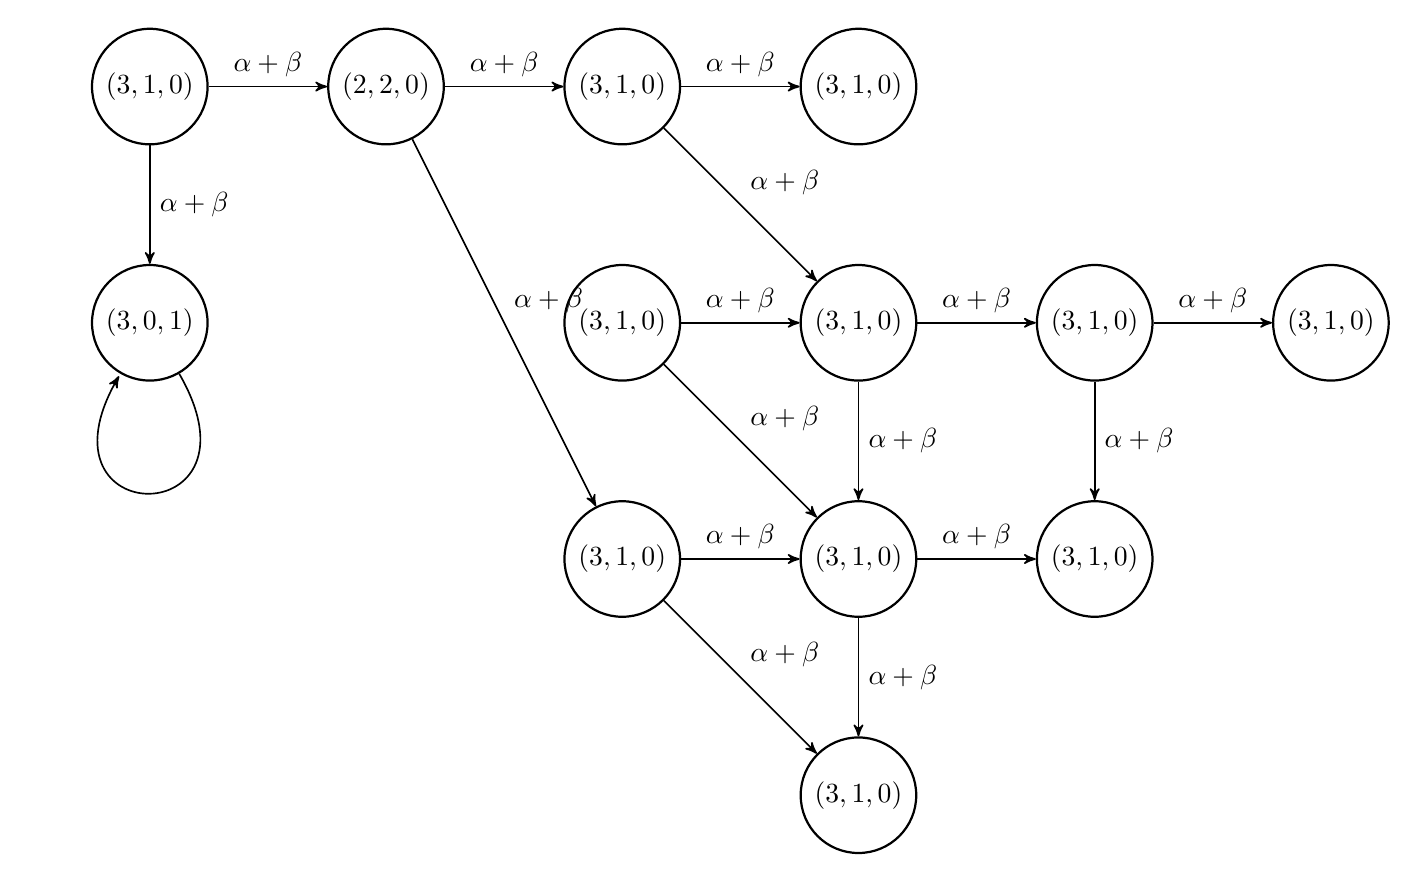
\begin{tikzpicture}[->, >=stealth', auto, semithick, node distance=3cm]
        \tikzstyle{every state}=[fill=white,draw=black,thick,text=black]
        \node[state]    (Init)                      {$(3,1,0)$};
        \node[state]    (S_301)[below of=Init]      {$(3,0,1)$};
        \node[state]    (S_220)[right of=Init]      {$(2,2,0)$};
        \node[state]    (D)[right of=S_220]         {$(3,1,0)$};
        \node[state]    (E)[below of=D]         {$(3,1,0)$};
        \node[state]    (F)[below of=E]         {$(3,1,0)$};
        \node[state]    (G)[right of=D]         {$(3,1,0)$};
        \node[state]    (H)[below of=G]         {$(3,1,0)$};
        \node[state]    (I)[below of=H]         {$(3,1,0)$};
        \node[state]    (J)[below of=I]         {$(3,1,0)$};
        \node[state]    (K)[right of=H]         {$(3,1,0)$};
        \node[state]    (L)[right of=I]         {$(3,1,0)$};
        \node[state]    (M)[right of=K]         {$(3,1,0)$};
        \path
        (Init) edge node{$\alpha + \beta$} (S_301)
            edge node{$\alpha + \beta$} (S_220)
        (S_301) edge [in=240,out=300,loop]  ()
        (S_220) edge node{$\alpha + \beta$} (D)
            edge node{$\alpha + \beta$} (F)
        (D) edge node{$\alpha + \beta$} (G)
            edge node{$\alpha + \beta$} (H)
        (E) edge node{$\alpha + \beta$} (H)
            edge node{$\alpha + \beta$} (I)
        (F) edge node{$\alpha + \beta$} (I)
            edge node{$\alpha + \beta$} (J)
        (H) edge node{$\alpha + \beta$} (K)
            edge node{$\alpha + \beta$} (I)
        (I) edge node{$\alpha + \beta$} (L)
            edge node{$\alpha + \beta$} (J)
        (K) edge node{$\alpha + \beta$} (M)
            edge node{$\alpha + \beta$} (L);
        \end{tikzpicture}
    \caption{$SIR(3,1,0)$ CTMC model with parameters$(\alpha, \beta)$}
\end{figure}

Uniformize the chain with uniformization rate $(3\alpha + 4\beta)$, we derive the following uniformized DTMC:
\begin{figure}
    \centering
    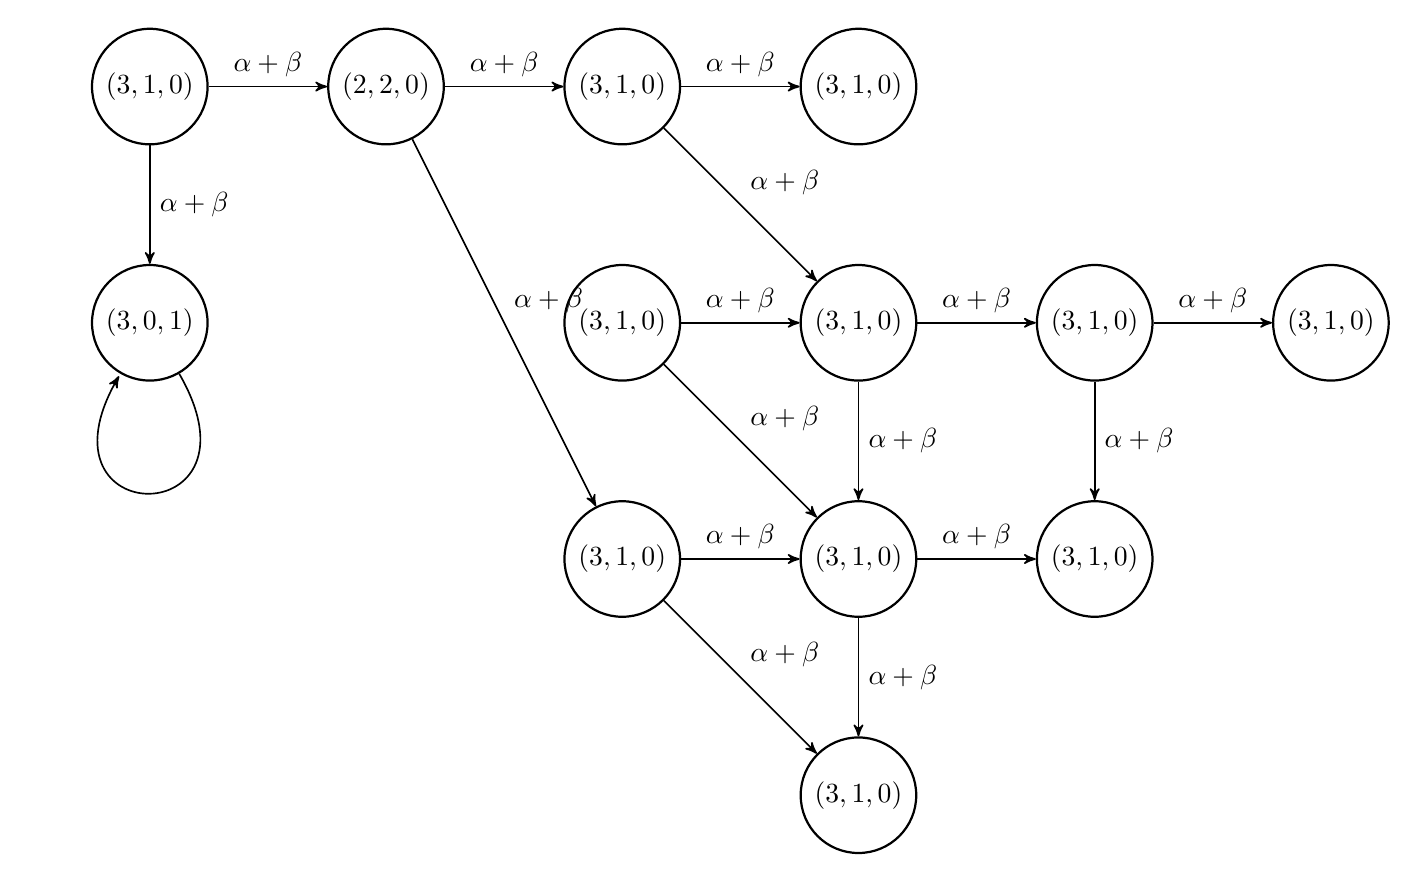
\begin{tikzpicture}[->, >=stealth', auto, semithick, node distance=3cm]
        \tikzstyle{every state}=[fill=white,draw=black,thick,text=black]
        \node[state]    (Init)                      {$(3,1,0)$};
        \node[state]    (S_301)[below of=Init]      {$(3,0,1)$};
        \node[state]    (S_220)[right of=Init]      {$(2,2,0)$};
        \node[state]    (D)[right of=S_220]         {$(3,1,0)$};
        \node[state]    (E)[below of=D]         {$(3,1,0)$};
        \node[state]    (F)[below of=E]         {$(3,1,0)$};
        \node[state]    (G)[right of=D]         {$(3,1,0)$};
        \node[state]    (H)[below of=G]         {$(3,1,0)$};
        \node[state]    (I)[below of=H]         {$(3,1,0)$};
        \node[state]    (J)[below of=I]         {$(3,1,0)$};
        \node[state]    (K)[right of=H]         {$(3,1,0)$};
        \node[state]    (L)[right of=I]         {$(3,1,0)$};
        \node[state]    (M)[right of=K]         {$(3,1,0)$};
        \path
        (Init) edge node{$\alpha + \beta$} (S_301)
            edge node{$\alpha + \beta$} (S_220)
        (S_301) edge [in=240,out=300,loop]  ()
        (S_220) edge node{$\alpha + \beta$} (D)
            edge node{$\alpha + \beta$} (F)
        (D) edge node{$\alpha + \beta$} (G)
            edge node{$\alpha + \beta$} (H)
        (E) edge node{$\alpha + \beta$} (H)
            edge node{$\alpha + \beta$} (I)
        (F) edge node{$\alpha + \beta$} (I)
            edge node{$\alpha + \beta$} (J)
        (H) edge node{$\alpha + \beta$} (K)
            edge node{$\alpha + \beta$} (I)
        (I) edge node{$\alpha + \beta$} (L)
            edge node{$\alpha + \beta$} (J)
        (K) edge node{$\alpha + \beta$} (M)
            edge node{$\alpha + \beta$} (L);
        \end{tikzpicture}
    \caption{$SIR(3,1,0)$ CTMC model with parameters$(\alpha, \beta)$}
\end{figure}
\subsection{Properties}
\subsection{Evaluation}



\chapter{Conclusion}
\section{Summary}

\begin{itemize}
    \item
\end{itemize}

\section{Future works}

\printbibliography
\end{document}